\pdfminorversion=7
\documentclass[journal]{IEEEtran}

\usepackage{microtype}
\usepackage{graphicx}
\usepackage[table]{xcolor}
\usepackage[caption=false,font=footnotesize]{subfig}
\usepackage{booktabs}
\usepackage{hyperref}
\usepackage{adjustbox}
\usepackage{tabularx}
\usepackage{enumitem}
\usepackage{amsmath}
\usepackage{mathtools}
\hypersetup{hidelinks}

\newcommand{\systemname}{DynaExQ}
\newif\ifartifactverified
% Set true only after scripts/audit_paper_results.py passes on the complete
% table/figure manifest.
\artifactverifiedfalse
\newcommand{\registeredperformancegraphic}[2][]{%
  \ifartifactverified
    \includegraphics[#1]{#2}%
  \else
    \fbox{\parbox[c][0.72in][c]{0.84\linewidth}{%
      \centering\scriptsize Registered performance artifact pending}}%
  \fi
}

\title{\systemname: Budget-Safe Online Precision Residency for Single-GPU MoE Inference}

\author{Kexin Chu, Dawei Xiang, and Wei Zhang%
\thanks{The authors are with the University of Connecticut, Storrs, CT 06269
USA (e-mail: kexin.chu@uconn.edu; ieb24002@uconn.edu;
wei.13.zhang@uconn.edu). Corresponding author: Wei Zhang.}}

\begin{document}

\maketitle

\begin{abstract}
Large Mixture-of-Experts (MoE) models are difficult to serve on one GPU because all expert weights must remain addressable although each token activates only a small subset. Offloading reduces resident memory but can expose PCIe transfers when batched routing produces a dense expert working set. Uniform post-training quantization avoids transfers but cannot reassign its limited high-precision capacity when routing distributions change. \systemname\ instead treats expert precision residency as online resource allocation under an explicit expert-memory budget. A routing-driven policy selects high-traffic experts, while an admission-controlled transition mechanism copies prepared precision versions on a separate CUDA stream and publishes a new expert handle only after transfer completion. Partitioned fixed-block pools bound the runtime-owned resident and in-flight transition footprint. Across three MoE models and six workloads, \systemname\ recovers up to 79\% of the quality gap between uniform INT2 and INT4. Performance experiments compare its fully resident execution against uniform PTQ on all models and the pinned official MoE-Infinity runtime on the supported Qwen3-30B model. Component studies quantify the effects of online selection, asynchronous transitions, hysteresis, and the high-precision budget.
\end{abstract}

\begin{IEEEkeywords}
Mixture-of-Experts, large language model inference, GPU memory management, mixed-precision quantization, runtime systems
\end{IEEEkeywords}

\ifartifactverified\else
\begin{center}
\colorbox{red!12}{\parbox{0.94\linewidth}{\centering\textbf{Internal draft.}
Result provenance is incomplete; this PDF is not submission-ready.}}
\end{center}
\fi

\section{Introduction}

Mixture-of-Experts (MoE) models~\cite{shazeer2017outrageously} scale neural-network capacity by routing each token to a small subset of expert subnetworks, keeping per-token compute bounded while the full parameter set must stay accessible for unconstrained routing. Modern MoE language models such as Mixtral~\cite{jiang2024mixtral}, DeepSeek-V2~\cite{deepseekv2}, and Qwen3~\cite{qwen3technicalreport} contain tens to hundreds of billions of parameters, yet activate only a few billion per token. Deploying these models on a single high-end GPU exposes a fundamental hardware constraint: device high-bandwidth memory (HBM), typically 48--80\,GB, must simultaneously hold expert weights, non-expert parameters, activations, the KV cache, and runtime buffers. Qwen3-Next-80B, for instance, requires roughly 160\,GB in FP16, far exceeding the HBM capacity of current accelerators. The deployment bottleneck is therefore not peak arithmetic throughput but \emph{on-device memory management}: deciding which expert weights remain resident, at what precision, and how residency adapts as the workload changes.

Two families of techniques address this memory-capacity wall.
The first, expert offloading and prefetching~\cite{li2023adaptive,yi2023edgemoe,xue2024moe,eliseev2023fast,hwang2024pre,zhong2024adapmoe,tang2024hobbit,song2024promoe,shen2025expertflow}, treats GPU HBM as a managed cache and moves experts across the PCIe memory hierarchy on demand.
The second, post-training quantization (PTQ)~\cite{lin2024awq,frantar2022gptq,kim2023mixturequantizedexpertsmoqe,duanmu2025mxmoe}, compresses expert weights to low bit-widths, reducing the per-expert device-memory footprint so the full pool fits on-chip.

Offloading works well when each iteration touches a small, stable expert subset. In practice, MoE activation becomes substantially denser during prefill and at larger batch sizes (\autoref{tab:expert_activation_ratio}), expanding the per-iteration working set beyond what can be staged within the PCIe compute-transfer overlap window. Once that window is exceeded, data movement stalls the GPU compute pipeline and amplifies worst-case latency (\autoref{fig:waiting-vs-prompt}).\looseness=-1

PTQ avoids cross-tier data movement entirely and, with no ongoing migration, achieves the lowest raw per-step latency. However, most PTQ pipelines fix a uniform or per-expert precision map offline. Expert utilization is heavy-tailed and task-dependent: the identity of frequently activated experts shifts across text, math, and code workloads (\autoref{fig:expert-active}). A static precision map therefore wastes scarce HBM capacity on experts that carry little traffic in the current task while over-compressing those that become critical. This paper does not claim to beat static PTQ on raw latency; it targets a better \emph{accuracy--throughput--memory} tradeoff under the same fixed device-memory budget.

We propose \systemname, which manages expert precision as a dynamically allocated on-device resource for single-GPU MoE inference under a declared HBM envelope. During inference, the system observes router outputs, estimates which experts carry disproportionate traffic over a stable time horizon, and allocates a limited high-precision budget to those experts. The remaining experts stay at lower precision. Preallocated pools and admission control keep all runtime-owned expert and transition memory within the envelope; the end-to-end cap holds when the deployment's KV-cache and activation reservations are respected.

The design separates policy from mechanism. A scheduler periodically selects budget-feasible high-precision sets per layer. A transition pipeline carries out promotions and demotions on a dedicated CUDA stream without blocking the forward path. Pool-based memory management with admission control prevents budget violations. Section~\ref{sec:design} describes each component.

The main contributions of this work are:
\begin{itemize}[leftmargin=1.5em, itemsep=1pt, topsep=2pt]
  \item We formulate single-GPU MoE inference under a hard device-memory constraint as an on-device precision residency management problem, targeting the accuracy--throughput--memory tradeoff rather than minimum raw latency alone.
  \item We design an asynchronous runtime execution model with versioned expert handles. A new handle is published only after its copy completes, and read leases plus per-compute-stream last-use events protect the old block until every dispatch and kernel that can reference it has drained.
  \item We introduce deterministic, pool-based device-memory management with admission control. Exact expert-sized blocks eliminate variable-size external fragmentation, per-tier capacities isolate resident slots, and a budget tracker prevents transient over-commitment during concurrent migrations.
  \item We evaluate \systemname\ on Qwen3-MoE-30B, Qwen3-Next-80B, and Phi-3.5-MoE across six benchmarks. \systemname\ recovers up to 79\% of the INT2-to-INT4 accuracy gap on Qwen3-Next-80B, from 73.58\% to 77.15\%. Performance experiments use uniform PTQ on all models and the pinned official MoE-Infinity runtime where its public implementation supports the evaluated model; ablations isolate each mechanism, and raw peak-memory traces test the 48\,GB deployment envelope.
\end{itemize}

\section{Background and Motivation}

\subsection{MoE Inference on a Single GPU}
On a single accelerator, expert weights dominate the memory footprint; they comprise roughly 95--96\% of the parameters in the three models studied here~\cite{qwen3technicalreport,qwen3nextmodelcard,abdin2024phi3}. Whether a model fits on-chip depends on how those weights are stored. Expert utilization is also inherently uneven: a small hot set receives a disproportionate share of traffic, so allocating equal fidelity to every expert is rarely cost-effective under a tight memory envelope.

\subsection{Offloading and Prefetching}
\label{sec:background-offload}
A family of systems treats GPU memory as a managed cache and fetches experts on demand~\cite{li2023adaptive,yi2023edgemoe,xue2024moe,eliseev2023fast,hwang2024pre,zhong2024adapmoe,tang2024hobbit,song2024promoe,kong2024swapmoe,shen2025expertflow}. Their opportunity for overlap depends on the size and predictability of the active set. We define instantaneous density as the number of unique selected experts per MoE layer, measured over all nonpadding tokens in a 2,048-token-capped prefill or over the immediately following one-token decode. Each table entry averages five deterministic prompt blocks and all routed layers; batch-$b$ uses the first $b$ prompts of the same 32-prompt block. \autoref{tab:expert_activation_ratio} shows that density rises with batch size: for Qwen3-30B at batch~32, prefill selects 94.0\% of experts and the next decode step selects 26.0\%. Measuring one decode step avoids conflating instantaneous demand with the union accumulated over a long generation. To quantify the transfer consequence in isolation, \autoref{fig:waiting-vs-prompt} replays measured per-layer active sets from a cold cache and serially copies each missed expert from pinned host memory. This microbenchmark reports exposed transfer time for blocking on-demand movement; it is not an end-to-end measurement of an overlapping offload system.

\begin{center}
\colorbox{gray!10}{%
\parbox{0.96\linewidth}{%
\textbf{Observation 1.}
Prefill and larger batches can activate a substantial fraction of the expert pool. A larger instantaneous working set reduces the transfer slack available to an offload cache and increases the cost of misses.}}
\end{center}

\begin{table}[t]
  \centering
  \caption{Mean unique-expert activation ratio (\%) across routed layers and five prompt blocks.}
  \label{tab:expert_activation_ratio}
  \vspace{-0.5em}
  \setlength{\tabcolsep}{3.5pt}
  \begin{tabularx}{\columnwidth}{@{}Xlrrrrrr@{}}
    \toprule
    \textbf{Model} & \textbf{Stage} & \textbf{bs=1} & \textbf{2} & \textbf{4} & \textbf{8} & \textbf{16} & \textbf{32} \\
    \midrule
    Qwen3-30B  & Decode & 6.3 & 7.9 & 11.8 & 16.1 & 20.8 & 26.0 \\
               & Prefill & 59.8 & 70.0 & 82.9 & 89.7 & 92.4 & 94.0 \\
    \midrule
    Qwen3-Next-80B & Decode & 1.9 & 3.7  & 6.7  & 14.9 & 25.4 & 39.2 \\
               & Prefill & 24.6 & 35.3 & 48.8 & 67.1 & 78.9 & 86.2 \\
    \midrule
    Phi-3.5-MoE & Decode & 12.5 & 22.7 & 37.1 & 59.3 & 77.8 & 88.8 \\
                & Prefill & 98.2 & 98.8 & 99.4 & 99.8 & 99.9 & 100.0 \\
    \bottomrule
  \end{tabularx}
\end{table}

\begin{figure}[t]
    \centering
    
\includegraphics[width=0.99\columnwidth]{figures/waiting_latency_vs_prompt_length.pdf}
    \caption{Mean exposed transfer time for cold-cache, trace-driven blocking expert offload on one RTX~A6000 (10 measured trials after two warmups per point).}
    \label{fig:waiting-vs-prompt}
    \vspace{-1.5em}
\end{figure}

\subsection{Static Post-Training Quantization}
\label{sec:background-ptq}

PTQ compresses weights to low bit-widths without retraining. General-purpose schemes such as GPTQ~\cite{frantar2022gptq}, AWQ~\cite{lin2024awq}, SmoothQuant~\cite{xiao2023smoothquant}, and LLM.int8()~\cite{dettmers2022gptint8} have been extended to MoE-specific settings~\cite{kim2023mixturequantizedexpertsmoqe,duanmu2025mxmoe,zhang2025moqe}, where routing imbalance and heterogeneous expert sensitivity motivate per-expert or per-block bit allocation. Once deployed, PTQ incurs no precision-migration traffic. Most pipelines nevertheless fix their precision map during calibration, implicitly treating the resulting expert ranking as stable at inference time.

\begin{figure*}[t]
    \centering
    \begin{minipage}{0.32\linewidth}
        \centering
        \subfloat[WikiText]{%
            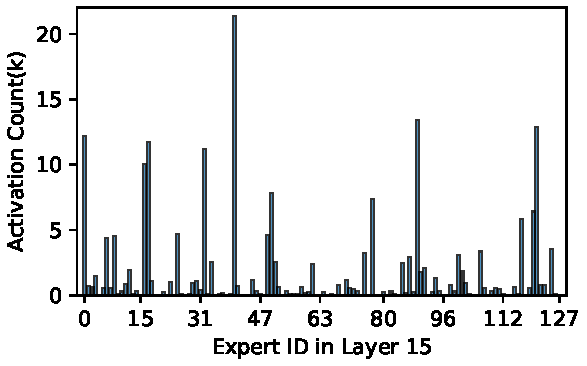
\includegraphics[width=0.95\linewidth]{figures/wikitext_thinking_on_layer_15.pdf}
        }
    \end{minipage}
    \begin{minipage}{0.32\linewidth}
        \centering
        \subfloat[GSM8K]{%
            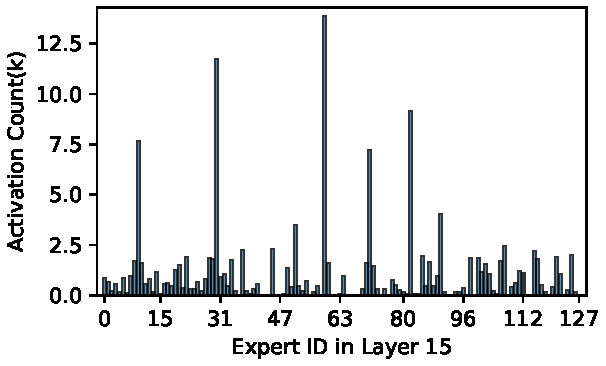
\includegraphics[width=0.95\linewidth]{figures/gsm8k_thinking_off_layer_15.pdf}
        }
    \end{minipage}
    \begin{minipage}{0.32\linewidth}
        \centering
        \subfloat[HumanEval]{%
            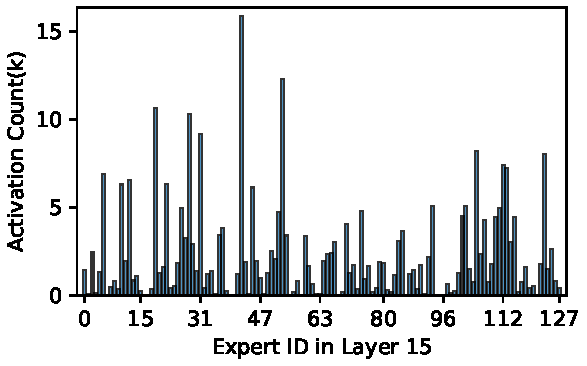
\includegraphics[width=0.95\linewidth]{figures/humaneval_thinking_on_layer_15.pdf}
        }
    \end{minipage}
    \caption{Selected token--expert dispatch counts at Layer~15 of Qwen3-MoE-30B under the full pinned WikiText, GSM8K, and HumanEval workloads. The scheduler is frozen with all experts at INT4; the top-10 most frequently selected experts are entirely disjoint across text, math, and code tasks.}
    \label{fig:expert-active}
    \vspace{-1.0em}
\end{figure*}

That assumption is brittle for MoE. Expert utilization is heavy-tailed and the identity of hot experts shifts across workloads (\autoref{fig:expert-active}). We count every selected top-$k$ token--expert dispatch, rather than thresholding router probabilities, and reset the counter between the three full evaluation workloads. Under this pinned protocol, the top-10 most frequently selected experts for text, math, and code are entirely disjoint.

\begin{center}
\colorbox{gray!10}{%
\parbox{0.96\linewidth}{%
\textbf{Observation 2.}
MoE expert usage is heavy-tailed and workload-dependent: a small set receives much of the traffic, but its membership changes across tasks. A precision map optimized for one routing distribution can therefore become stale.}}
\end{center}

\subsection{Motivation and Challenges for Online Precision Control}
\label{sec:background-motivation}

The observations above suggest adapting expert precision online under a strict GPU budget. A natural concern is whether such adaptation destabilizes quality. We concatenate the pinned WikiText-2 test split and measure perplexity over at most 128 exact 2,048-token windows while increasing the fraction of low-precision experts per layer. We obtain one expert ranking from the independent calibration corpus, freeze online reassignment, and demote an exact suffix of that same ranking at every point; thus, the sweep isolates the precision quota rather than conflating it with scheduler adaptation. As \autoref{fig:ppl} shows, when demotion targets infrequently activated experts first, perplexity rises smoothly.

\begin{center}
\colorbox{gray!10}{%
\parbox{0.96\linewidth}{%
\textbf{Observation 3.}
When demotion follows a fixed cold-to-hot ranking, perplexity changes smoothly with the low-precision quota. Expert precision therefore exposes a controllable quality--memory tradeoff.}}
\end{center}

\begin{figure}[t]
    \centering
    \begin{minipage}{0.46\linewidth}
        \centering
        \subfloat[Qwen3-30B]{%
            
\includegraphics[width=0.95\linewidth]{figures/wiki_ppl_qwen30b.pdf}
        }
    \end{minipage}
    \begin{minipage}{0.46\linewidth}
        \centering
        \subfloat[Qwen3-Next-80B]{%
            
\includegraphics[width=0.95\linewidth]{figures/wiki_ppl_qwen80b.pdf}
        }
    \end{minipage}
    \caption{Perplexity vs.\ low-precision expert ratio (Qwen3-30B: FP16 vs.\ INT4; Qwen3-Next-80B: INT4 vs.\ INT2).}
    \label{fig:ppl}
    \vspace{-1em}
\end{figure}

Realizing this tradeoff at runtime, however, requires satisfying three constraints:
\begin{itemize}[leftmargin=1.5em, itemsep=1pt, topsep=2pt]
    \item \textbf{Hard expert-budget invariance.} Precision changes alter the resident footprint. The runtime must never exceed the device envelope allocated to expert residency and transitions; otherwise out-of-memory failures or forced evictions cascade into instability. The deployment must separately size KV-cache and activation reserves for its supported request shape.
    \item \textbf{Critical-path isolation.} Precision transitions involve heavyweight device transfers that must not stall the forward pass.
    \item \textbf{Tail-latency robustness.} Naive reallocation can thrash when routing scores fluctuate, amplifying migration traffic and widening P99 latency.
\end{itemize}

\section{\systemname\ Architecture}
\label{sec:design}

\systemname\ treats expert precision as an online, budget-constrained resource. Each expert has prepared lower- and higher-precision host representations, denoted $b^{\text{lo}}$ and $b^{\text{hi}}$. Exactly one representation is published for device dispatch; a bounded staging copy may coexist only while a transition is in flight. The runtime changes which experts occupy $b^{\text{hi}}$ subject to three constraints: (C1)~budget feasibility, (C2)~no explicit transition synchronization on the forward path, and (C3)~stability under routing fluctuations.

\begin{figure*}[t]
    \centering
    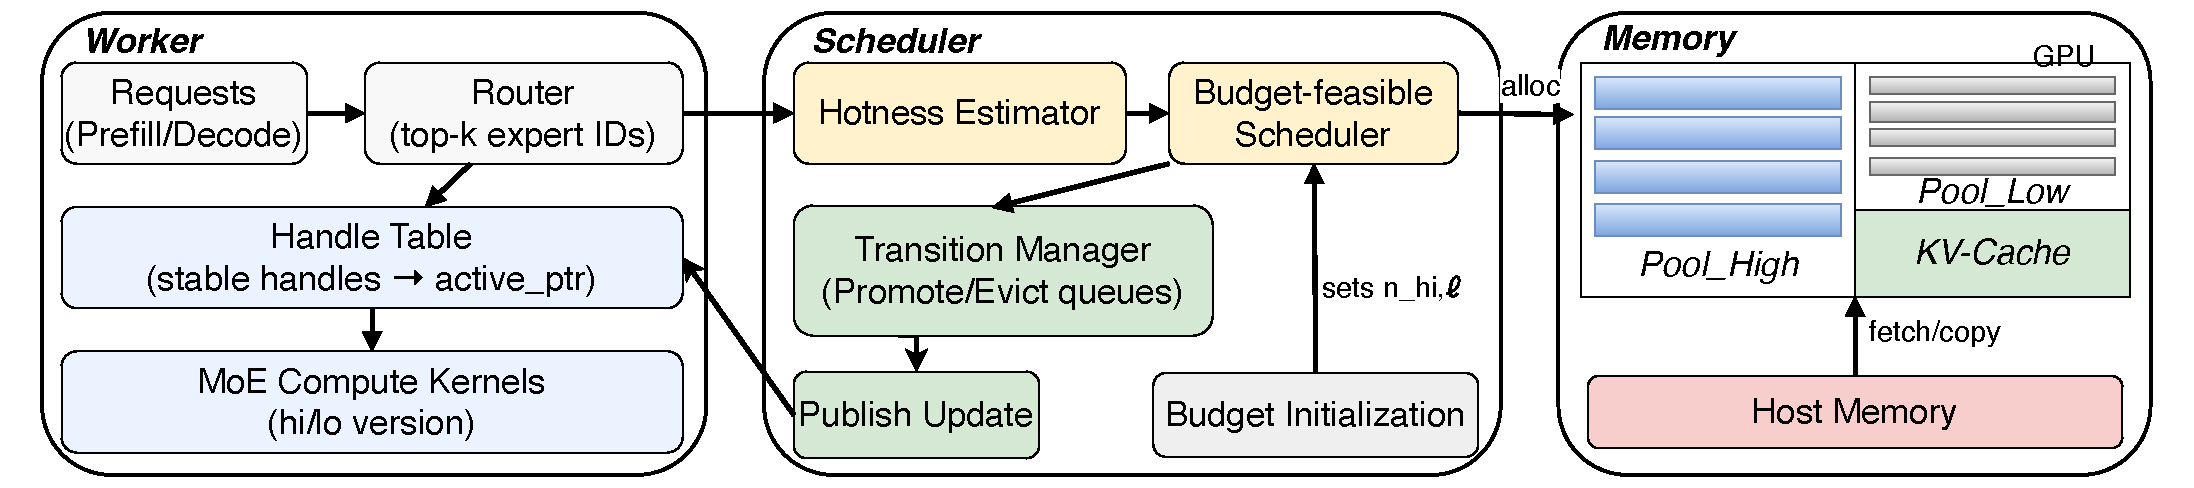
\includegraphics[width=0.93\linewidth]{figures/dynaexq_arch.pdf}
    \caption{System architecture of \systemname. The worker resolves a versioned expert handle; a scheduler observes router traces and updates precision residency under a strict HBM budget; a transition pipeline carries out promotions and demotions on a dedicated migration stream.}
    \label{fig:architecture_overview}
    \vspace{-1em}
\end{figure*}

\subsection{Architecture Overview and Execution Model}
\label{sec:overview}

\autoref{fig:architecture_overview} shows the end-to-end control loop. The design separates \emph{policy} (what to change) from \emph{mechanisms} (how to change safely).

\paragraph{Policy.}
The scheduler interprets router-derived traffic and chooses a budget-feasible high-precision resident set per layer: hotness estimation via periodic aggregation, top-$n$ selection under fixed per-layer capacities, and hysteresis to damp oscillation. It emits target sets and promotion/demotion candidates but does not allocate GPU memory directly.

\paragraph{Mechanisms.}
Three mechanisms implement this runtime execution model:
(i)~versioned, representation-immutable per-expert handles with publish-after-complete semantics isolate dispatch from in-flight data movement;
(ii)~partitioned device pools and a budget tracker admit or reject each transition before any allocation;
(iii)~an asynchronous transition pipeline runs data movement on a dedicated CUDA stream and publishes a new handle only after transfer completes.
Consequently, transition submission does not wait for a copy, dispatch cannot observe a partially populated buffer, and no transition starts without a prior reservation against the declared HBM envelope. Stream separation does not eliminate memory-bandwidth contention, which we measure end to end.

\paragraph{Worker-side dispatch.}
On the worker side, each request invokes the router to obtain top-$k$ expert IDs. Each ID resolves to a versioned handle containing a fully materialized device block and its quantization metadata. Dispatch observes either the previous complete handle or the next complete handle; it does not mutate a handle in place.

\paragraph{Scheduler-side control.}
The scheduler consumes router traces asynchronously. Per-expert hotness statistics feed a budget-feasible selection that determines, for each layer~$\ell$, a high-precision resident set subject to a layer capacity $n_{\mathrm{hi},\ell}$. The resulting target sets drive a transition manager that maintains promote/evict queues and issues background work on a migration stream.

\paragraph{Budget initialization.}
Before inference, the system derives per-layer capacities $\{n_{\mathrm{hi},\ell}\}$ from total device memory $M_{\text{total}}$. Let $M_{\text{fixed}}$ reserve non-expert parameters, activations, KV cache, conversion workspace, and a safety margin. Let $M_{\text{trans}}$ be preallocated headroom for at most $K$ simultaneous publish-before-reclaim transitions, and let $m^{\text{hi}}_\ell$ and $m^{\text{lo}}_\ell$ be the measured packed bytes of one expert at each tier in layer~$\ell$. Initialization chooses capacities satisfying
\begin{equation}
\begin{aligned}
M_{\text{resident}}
&=\sum_{\ell}\!\left[n_{\mathrm{hi},\ell}m^{\text{hi}}_\ell+
(E_{\ell}-n_{\mathrm{hi},\ell})m^{\text{lo}}_\ell\right],\\
M_{\text{trans}}
&=K\max_{\ell,b\in\{\mathrm{hi},\mathrm{lo}\}}m^b_\ell,\\
M_{\text{resident}}+M_{\text{trans}}
&\le M_{\text{total}}-M_{\text{fixed}}.
\end{aligned}
\label{eq:hbm-budget}
\end{equation}
where $E_\ell$ is the routed-expert count in layer~$\ell$. The implementation supports uniform, expert-count-proportional, and greedy capacity allocation; the evaluation uses deterministic proportional allocation. An independent train/validation calibration trace first runs the all-low configuration and ranks experts by mean routed probability mass across prompts. This FP64 accumulator is order-invariant, unlike the online EMA, and avoids initializing from an arbitrary expert-ID prefix. The first $n_{\mathrm{hi},\ell}$ ranked experts populate the initial higher-precision set; sensitivity experiments vary only this prefix length. Each artifact binds the checkpoint, calibration-source hash, selected prompt identifiers, aggregation rule, ranking hash, and clean code revision. After initialization, $n_{\mathrm{hi},\ell}$ remains fixed and only expert \emph{identities} change online.

\paragraph{Scope of the memory invariant.}
Equation~\eqref{eq:hbm-budget} is enforced exactly for memory owned by \systemname: resident expert blocks, staging blocks, and conversion workspace are allocated or reserved at startup, and no transition is admitted beyond those capacities. The whole-process HBM cap additionally assumes that KV cache, activation, and framework allocations remain within their declared reservations. Startup checks available HBM against all declared components, but the prototype does not intercept a framework allocator if a later request exceeds its KV or activation reserve. We report both the expert-pool counters and the observed process peak to distinguish the enforced invariant from this deployment assumption.

\subsection{Online Scheduling Policy}
\label{sec:policy}

The scheduling policy determines which experts should occupy the limited high-precision capacity. It is kept simple so that its behavior is easy to reason about and its per-tick cost stays small relative to inference.

\paragraph{Hotness estimation.}
For a forward step with $N_\ell$ routed token positions, let $p_{\ell,t,e}$ be the router probability for expert $e$ when it is selected in the top-$k$ set $\mathcal{R}_{\ell,t}$, and zero otherwise. The runtime uses the selected probability mass per token,
\[
c_{\ell,e}=\frac{1}{N_\ell}\sum_{t=1}^{N_\ell}
\mathbf{1}[e\in\mathcal{R}_{\ell,t}]\,p_{\ell,t,e}.
\]
Thus the signal captures both selection frequency and router confidence. Updates are applied after every observation, with $c_{\ell,e}=0$ for unselected experts so stale scores decay. Residency decisions are triggered every $T_u$ forward steps; the step-based definition is deterministic under replay and makes the number of router observations per decision explicit. The smoothed hotness score is:
\[
S_{\ell,e} \leftarrow \alpha \cdot S_{\ell,e} + (1-\alpha)\cdot c_{\ell,e},
\]
where $\alpha \in [0,1)$ controls how quickly past observations decay. This construction uses router outputs only and requires no labels or online quality signals.

\paragraph{Budget-feasible selection.}
For each layer $\ell$ with capacity $n_{\mathrm{hi},\ell}$, the high-precision set is:
\[
H_\ell \leftarrow \mathrm{TopN}\!\left(\{S_{\ell,e}\}_e,\; n_{\mathrm{hi},\ell}\right).
\]
Selection is local to each layer and budget-feasible by construction: no cross-layer coordination is needed. The set difference against the current resident set yields promotion candidates $H_\ell \setminus H_\ell^{\mathrm{cur}}$ and demotion candidates $H_\ell^{\mathrm{cur}} \setminus H_\ell$. These candidates are passed to the transition pipeline, which admits promotions only when the budget tracker can reserve the required memory (Section~\ref{sec:memmgmt}).

\paragraph{Hysteresis for stability.}
A plain top-$N$ rule can cause unnecessary churn when several experts have similar hotness scores. Each swap triggers a promotion and a matching demotion, consuming migration bandwidth without improving quality. We therefore apply additive-margin hysteresis: after the cold-start set reaches capacity, the highest-scoring outsider replaces the lowest-scoring incumbent only when their score difference exceeds $\delta$. Candidate pairs are processed in score order until the inequality fails. Hysteresis does not change the budget constraint; it reduces oscillations and makes the transition rate more predictable under transient routing fluctuations.

The policy produces a target set per layer at cadence $T_u$. A target does not become visible merely because it was selected: each expert dispatch continues to acquire the last published handle until that expert's pending version switch completes.

\subsection{GPU Memory Management}
\label{sec:memmgmt}

Dynamic residency stresses GPU memory in two ways. First, promotions and evictions allocate large weight buffers; if these share a general-purpose device heap with variable request sizes, external fragmentation and allocator jitter can inflate latency variance. Second, several transitions may overlap in time; if their aggregate footprint is unbounded, concurrent promotions can exhaust the device budget even when each is individually feasible.

\paragraph{Partitioned pools and fragmentation control.}
We divide the GPU memory assigned to expert weights into disjoint per-layer, per-tier pools: $\texttt{pool\_hi}$ for high-precision versions and $\texttt{pool\_lo}$ for low-precision versions. Their capacities are fixed independently of the logically reserved KV-cache and framework budgets. Within each pool, one fixed-size byte block stores one expert's measured packed representation. This eliminates variable-size external fragmentation and keeps the free/allocate path uniform, following the same principle as paged KV-cache memory in LLM inference engines~\cite{kwon2023vllm}. Each pool maintains its own free list, so transitions never invoke the general-purpose device allocator. Separating capacities by precision tier prevents churn in one tier from consuming blocks assigned to the other. Rapid promotions filling $\texttt{pool\_hi}$, for example, cannot encroach on $\texttt{pool\_lo}$'s resident set.

\paragraph{Budget model and admission.}
A \texttt{BudgetTracker} enforces the global memory budget through explicit reservation and release operations. The usable device memory $M_{\text{total}}$ is partitioned at startup into:
\begin{itemize}[leftmargin=1.5em, itemsep=0pt, topsep=2pt]
\item $M_{\text{fixed}}$: declared KV cache and activation reserves, measured non-expert model state, safety margin, and a conservative two-expert kernel-conversion workspace per admitted INT4 transition.
\item $M_{\text{exp,hi}}^{\text{cap}}$: cap on resident high-precision expert weights.
\item $M_{\text{exp,lo}}^{\text{cap}}$: cap on resident low-precision expert weights.
\item A global fixed-block staging pool for publish-before-reclaim overlap, so concurrent migration work is allocated and accounted for before it starts.
\end{itemize}
Every transition must call \texttt{try\_reserve} before entering the executor. Admission checks the destination-tier cap, the pending-transfer cap, and a cross-tier cap on all committed plus pending expert bytes. The scheduler emits a replacement as an indivisible pair and orders its demotion before its promotion; the global staging pool covers the publish-before-reclaim overlap. When the paired transition frees the destination layer's resident slot, the runtime copies any staging-backed handle into that slot and returns the transient block, preventing staging capacity from becoming long-lived residency. If admission or allocation fails, the request is rejected and reconsidered from the published state at a later tick. Because the device pools are preallocated and admission precedes allocation, concurrent requests cannot grow \systemname-owned HBM beyond the startup envelope.

\subsection{Asynchronous Transition Pipeline}
\label{sec:pipeline}

The transition pipeline performs data movement and pointer updates while the compute stream runs independently.

\paragraph{Versioned-handle publication.}
The registry maps each expert key to a versioned handle whose published representation fields (tier, block, and packed metadata) are never modified in place; only lease and last-use bookkeeping changes. Publication is a single dictionary replacement under the registry lock. Before issuing expert kernels, an adapter acquires a short read lease on the currently published object and releases it after recording the compute-stream event. A handle retains the latest event for each compute stream, bounding metadata by serving concurrency rather than request count. A monotonically increasing version lets adapters skip unchanged metadata refreshes. During promotion, the destination block is filled on the migration stream and the transition worker waits for its completion event before publishing the new handle. The reclaimer first waits for the old object's lease count to reach zero and then waits for all of its per-stream last-use events. This two-part fence covers the otherwise unsafe interval in which dispatch has read an old handle but has not yet launched its kernel.

\begin{figure}[t]
    \centering
    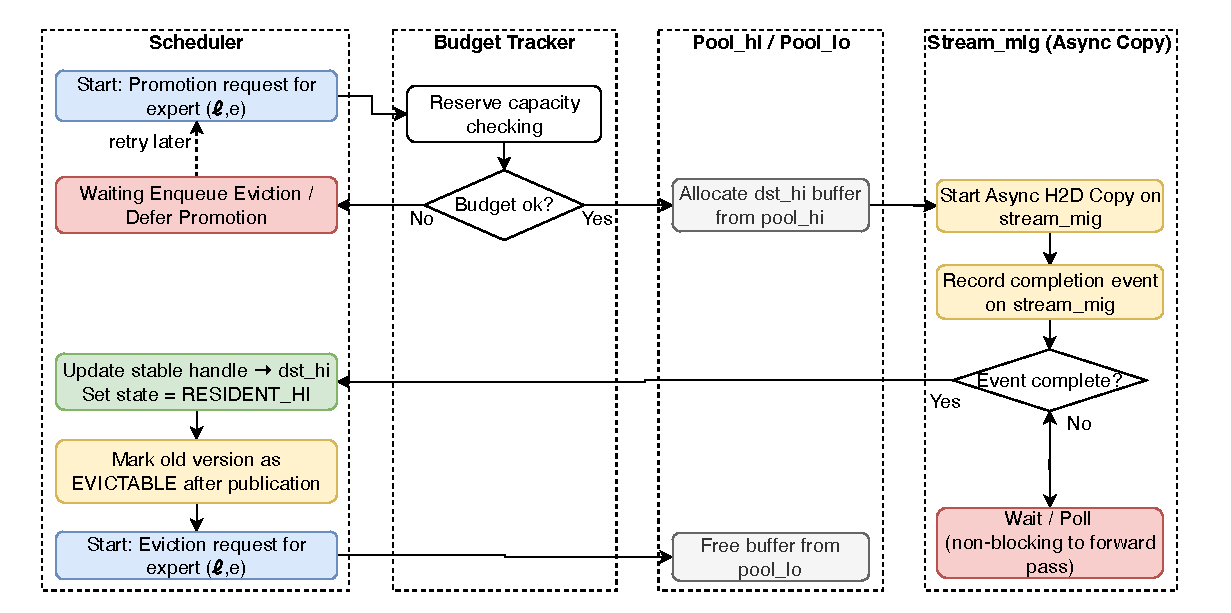
\includegraphics[width=0.99\columnwidth]{figures/dynaexq_procedure.pdf}
    \caption{Promotion and eviction procedure in the transition pipeline.}
    \label{fig:procedure}
    \vspace{-1em}
\end{figure}

\paragraph{Stream separation and backpressure.}
A bounded thread executor issues copies on a dedicated CUDA stream $\texttt{stream}_{\text{mig}}$, disjoint from the default compute stream used by attention and expert kernels. The scheduler keeps each replacement pair intact and submits its demotion first. Backpressure is implemented at admission: a request enters the executor only after passing the budget checks above. A rejected request is not reported as resident; the next decision is recomputed from a snapshot of actually published tiers.

\paragraph{Promotion procedure.}
For a target expert $(\ell,e)$, the pipeline proceeds as follows (\autoref{fig:procedure}):
\begin{enumerate}[leftmargin=1.5em, itemsep=0pt, topsep=2pt]
\item Obtain a successful \texttt{try\_reserve} for the high-precision footprint.
\item Allocate a destination buffer from $\texttt{pool\_hi}$, or from the bounded global staging pool if the resident slot is not yet reclaimable.
\item Issue an asynchronous copy from the pinned host representation on $\texttt{stream}_{\text{mig}}$.
\item Record a CUDA event on $\texttt{stream}_{\text{mig}}$.
\end{enumerate}
The registry publication executes only after the completion event fires, so dispatch never observes a partially populated buffer. The compute stream does not wait on the migration stream; a subsequent dispatch simply resolves the latest published handle.

\paragraph{Eviction procedure.}
When the scheduler marks an expert for demotion, the pipeline publishes the low-precision handle and then reclaims the high-precision buffer. The old handle's read leases close the read-before-launch race; its per-stream compute events then ensure no issued kernel is still reading the buffer before it returns to the pool.

\paragraph{Host-side weight preparation.}
Before timed inference, the prototype materializes both packed tiers in pinned host memory one layer at a time and releases that layer's native source parameters as soon as both versions are complete. This avoids holding the full source model and the full dual-tier cache simultaneously. It next populates every device-resident handle from the fixed pools. The untimed initialization still increases host DRAM demand but makes a measured transition a copy of an existing representation rather than first-use quantization. The experiment aborts if any expert cannot be cached, released, or registered; it never silently falls back to native weights.

\section{Implementation}
\label{sec:impl}

\systemname\ is implemented in Python and PyTorch~\cite{paszke2019pytorch} and integrates with Hugging Face Transformers~\cite{wolf2020transformers}. The implementation is divided into a model-independent control plane and thin model adapters. This separation keeps scheduling and memory-safety logic independent of a particular router or expert MLP layout.

\subsection{Control Plane}

\paragraph{Observation and scheduling.}
Model adapters report the router's top-$k$ expert identifiers and routing weights to a \texttt{RouterObserver}. A \texttt{HotnessTracker} accumulates per-layer counters and updates the EMA state. At a scheduling tick, \texttt{PrecisionScheduler} applies the per-layer capacity, hysteresis margin, and transition-rate limit to produce typed promotion and demotion requests. The scheduler never mutates a live expert handle.

The calibration entry point consumes at least 128 uniquely identified prompts from train, validation, development, or explicitly designated calibration splits; test splits are refused. It forces the all-low representation, disables online reassignment, and accumulates each prompt's token-normalized routed probability mass in a separate FP64 counter. Dividing by prompt count yields an order-invariant calibration score, while the FP32 EMA remains dedicated to online adaptation. The entry point emits a full stable ranking per layer and hashes both the source file and selected identifiers. Formal runs require this schema-v2 ranking artifact to match the exact checkpoint and model contract. The runtime records the realized prefix set, allowing the audit to prove that full, static, blocking, and sensitivity runs began from the intended common map.

\paragraph{Handles and transition lifecycle.}
\texttt{ExpertRegistry} stores one versioned handle per $(\ell,e)$ pair. A handle records its precision tier, packed quantization metadata, originating pool block, byte footprint, reservation, active-reader count, and latest event per compute stream. \texttt{TransitionEngine} uses a bounded worker pool to execute four stages: obtain the prepared host representation, reserve and allocate the destination block, copy the packed bytes, and publish the new handle. A failed reservation or exhausted pool leaves the previous handle active. After publication, the engine waits for all leases on the old object to drain and then for its per-stream last-use events before returning the block to its originating resident or global staging pool. If an adapter cannot provide a precise event, the implementation conservatively falls back to device synchronization; both paths are counted, and formal asynchronous artifacts require zero global-sync fallbacks.

\paragraph{Memory accounting.}
\texttt{BudgetTracker} maintains committed and pending bytes separately for the two precision tiers and enforces a cross-tier live-byte cap. Its \texttt{try\_reserve}, \texttt{commit}, and \texttt{release} operations are serialized by a lock, and a staging cap bounds pending work. The allocator pre-allocates disjoint per-layer, per-tier resident pools plus a global transient pool; transitions invoke no global device allocation. A compare-and-swap registry update repatriates staging-backed handles when the paired swap creates a resident hole. Because expert shapes may differ across models, block sizes and counts are derived from the packed representation rather than nominal bit width.

\subsection{Quantized Representations and Dispatch}

\paragraph{Packed representation.}
The quantization layer exposes a common \texttt{PackedTensor} abstraction for FP16, group-wise symmetric INT4 (128-weight groups), and group-wise symmetric INT2 (64-weight groups). It stores packed bytes, FP16 scales, tensor dimensions, group size, and the physical storage charged by admission control. Reference pack, unpack, and dequantize-then-GEMM paths support correctness testing. A compatibility backend invokes AutoRound's per-tensor symmetric quantizer and converts its output to the same representation; this path implements symmetric rounding, not AutoRound's activation-calibrated optimization loop.

\paragraph{Device kernels and workspace.}
INT4 dispatch uses PyTorch's fused int4pack matrix multiplication. INT2 dispatch uses a Triton kernel that unpacks values within the matrix multiplication and therefore avoids a full FP16 expert temporary. During an INT4 transition, the kernel-native layout replaces the canonical transfer layout within the same pool block, and its scale-and-zero storage remains charged to the handle. Conversion briefly creates a nibble-swapped input, a native-layout output, and scale/zero tensors. Startup consequently reserves a conservative two-expert INT4 conversion workspace per admitted transition before solving the resident allocation. Admission accounts for these physical layouts and workspaces, rather than nominal weight bits, and each artifact records the selected backend. A formal run aborts if the requested format lacks a device kernel that satisfies this envelope.

\paragraph{Model adapters.}
The Qwen3-MoE, Qwen3-Next, and Phi-3.5-MoE adapters acquire a handle immediately before routed-expert dispatch and release its lease after the final routed kernel. Gate, up, and down projections retain separate packed metadata but participate in one expert transition. Qwen3-MoE switches from Transformers' grouped-expert shortcut to handle-aware dispatch, because the shortcut bypasses per-expert resolution. Qwen3-Next's shared expert remains on the fixed dense path and is charged to the dense reservation. Once attached, an adapter fails closed on a missing or incomplete handle; native dispatch remains available only before attachment and in equivalence tests.

\paragraph{Startup path.}
Before a dynamic experiment, the runtime verifies that the declared layer count, routed-expert count, and top-$k$ match the checkpoint. It loads the source on CPU, packs both tiers in 16-expert chunks, releases native expert tensors layer by layer, and returns freed host arenas to the operating system. Only the remaining dense model is then moved to one specified GPU. Startup measures all remaining parameter and buffer bytes, raises an underestimated dense reservation, sizes conversion workspace from the chosen tier pair, and allocates the fixed pools. The run is rejected unless one device can hold the pools together with the declared KV-cache, activation, workspace, and safety reserves. Integration validation additionally requires that the attached model both emit routing observations and consume registered handles.

\subsection{Testing and Failure Semantics}

\paragraph{Correctness tests.}
CPU tests cover bit packing, quantization error, byte accounting, paired rate limiting, reservation races, global staging allocation, publish-after-copy ordering, lease-and-event-fenced reclamation, and repeated transitions without block leakage. Integration tests compare the Phi-MoE, Qwen3-MoE, and upstream Qwen3-Next adapters with native forward execution when handles reference equivalent weights. The Qwen3-Next test also verifies that releasing routed source tensors preserves its shared expert.

\paragraph{Experiment failure semantics.}
The evaluation CLI distinguishes incorrect model outputs from infrastructure failures and applies one named paper protocol. Paired comparisons require identical dataset fingerprints and sample identifiers before computing exact McNemar tests with Holm correction. The MoE-Infinity adapter binds the official repository commit, recursive source-tree manifest, and model snapshot, and accepts a run only when both offloaded expert state and measured prefetch activity are present. Transition artifacts record rejection causes, bytes copied, stage timings, pool occupancy, workspace reservations, and final budget counters.

During each formal timed generation, a 2\,ms NVML poller maps the selected CUDA device to its physical UUID and records current-process HBM use, including native allocations outside PyTorch's counters. Idle foreign HBM residency is recorded separately, while any observed foreign-process utilization invalidates the sample. Finally, a registrar hashes each artifact with its reproduction command. The manuscript audit enumerates every empirical and statistical claim and rejects missing, modified, dirty-tree, method-inconsistent, incompletely sampled, or memory-unaccounted evidence. Optional backends and large-model tests remain outside the default suite, so an unavailable quantizer or checkpoint cannot silently produce a passing experiment.

\section{Evaluation}

We evaluate \systemname\ under a 48\,GB single-GPU envelope. The study asks whether dynamic precision residency (1)~recovers quality lost to a fully resident low-precision baseline, (2)~maintains useful latency and throughput as routed activation becomes dense, (3)~benefits from each policy and mechanism component, and (4)~obeys its memory invariant across precision budgets. Static PTQ is the no-migration reference; an executable offloading system is included where its public implementation supports the evaluated checkpoint.

\subsection{Experimental Setup}
\label{sec:eval-setup}

\begin{table}[t]
  \centering
  \caption{Configuration of evaluated MoE models.}
  \label{tab:moe_config}
  \vspace{-0.5em}
  \setlength{\tabcolsep}{4pt}
  \resizebox{\linewidth}{!}{
  \begin{tabular}{lccc}
    \toprule
    & \textbf{Qwen3-30B} & \textbf{Qwen3-Next-80B} & \textbf{Phi-3.5-MoE} \\
    \midrule
    Total Parameters & 30.5B & 80B & 42B \\
    Activated / Token & 3.3B & 3B & 6.6B \\
    Reference Tier & FP16 & INT4 & FP16 \\
    Expert Weight Fraction & 95\% & 96\% & 96\% \\
    Layers & 48 & 48 & 32 \\
    Routed Experts / Layer & 128 & 512 (+1 shared) & 16 \\
    Top-$K$ & 8 & 10 & 2 \\
    \bottomrule
  \end{tabular}}
\end{table}

\noindent\textbf{Models.}
We use \nolinkurl{Qwen/Qwen3-30B-A3B-Instruct-2507}~\cite{qwen3technicalreport}, \nolinkurl{Qwen/Qwen3-Next-80B-A3B-Instruct}~\cite{qwen3nextmodelcard}, and \nolinkurl{microsoft/Phi-3.5-MoE-instruct}~\cite{abdin2024phi3} (\autoref{tab:moe_config}).

\noindent\textbf{Benchmarks.}
WikiText-2~\cite{merity2016pointer} (perplexity), MMLU-Pro~\cite{wang2024mmlu}, GPQA~\cite{rein2024gpqa}, AIME25~\cite{zhang2025aime25}, GSM8K~\cite{cobbe2021gsm8k}, and HumanEval~\cite{chen2021evaluating}.

\noindent\textbf{Evaluation protocol.}
We use the complete pinned test splits of MMLU-Pro and GSM8K, all 198 GPQA-Diamond questions, all 30 AIME25 problems, and all 164 HumanEval tasks. GPQA answer choices are shuffled once with seed 42 and the resulting order is shared by every method. Multiple-choice accuracy uses the conditional log-likelihood of each complete answer label rather than a single token; all labels for one question are scored in one unpadded batch so an online precision switch cannot occur between candidates. Numeric answers are taken from an explicit final-answer field, or from the last generated integer when the field is absent; matching an intermediate number does not count. HumanEval reports pass@1 only after executing the official tests with greedy decoding. WikiText perplexity is computed over at most 128 exact 2,048-token windows, with overlapping context labels masked when a shorter stride is used; each artifact stores every window boundary, effective target-token count, mean loss, and NLL so the aggregate can be independently recomputed. The five-task average is a descriptive effect size, not a pooled significance test. For paired method comparisons, we match sample identifiers and dataset fingerprints, apply an exact McNemar test to each task, and use Holm correction across the five tests.

\noindent\textbf{Hardware and stack.}
All experiments run on a single NVIDIA RTX~A6000 (48\,GB device memory). \systemname\ is integrated into a PyTorch/Transformers-based MoE inference stack~\cite{paszke2019pytorch,wolf2020transformers}. Hot routed experts use a higher-precision tier (FP16 for Qwen3-30B and Phi-3.5-MoE; INT4 for Qwen3-Next-80B); cold routed experts remain at a lower tier (INT4 or INT2, respectively). The Qwen3-Next shared expert remains fixed and is counted with non-routed weights.

\noindent\textbf{Measurement and provenance.}
Quality runs use greedy decoding with a fixed seed; each binomial accuracy or pass@1 result includes a 95\% Wilson interval in its artifact. Latency experiments use exact-length, non-padded 2,048-token inputs and generate 256 tokens per sequence, with five warmup iterations and 100 measured iterations; we report the mean, median, P95, and P99 from the raw samples. Model-level TTFT includes prefill and first-token selection, while TPOT covers subsequent cached decode steps. These measurements exclude request queueing, tokenization, network transport, and response serialization. During each timed generation, NVML samples whole-process HBM use on the selected GPU every 2\,ms, covering non-PyTorch CUDA allocations; raw PyTorch allocated/reserved high-water counters are retained separately. Every artifact records the checkpoint, method, quantization format, Git commit and dirty state, software versions, GPU model and UUID, seed, raw samples, memory-monitor metadata, and failed-example count. Dataset identity includes repository, configuration, split, immutable repository commit, source row count, and the loader's content fingerprint. A manuscript row is admitted only when all examples were evaluated and its values match the registered JSON artifact.

\noindent\textbf{Baselines.}
Static PTQ obeys the same single-GPU footprint; Qwen3-30B and Phi-3.5-MoE use uniform expert INT4. Qwen3-Next uses Intel's official mixed-AutoRound RTN checkpoint~\cite{autoround}: expert W4/group-128, non-expert W8, and FP16 gates. We content-pin ModelScope's moving ref through its complete path/size/hash catalog. Its low baseline deterministically reconstructs and repacks the same experts as symmetric W2/group-64, retaining all overrides. Thus the labels denote expert tiers; INT2 is requantized from INT4 and can incur compounded error.

For offloading, we pin the official MoE-Infinity repository and enable expert offload, activation-aware caching, and overlapping speculative prefetch on Qwen3-30B~\cite{xue2024moe,moeinfinityrepo}. Because the current public runtime differs from the paper implementation, we label it ``MoE-Infinity (open source).'' Its model adapters do not support the exact Qwen3-Next or Phi checkpoints used here, so the offloading comparison is limited to Qwen3-30B.

\subsection{Quality under a Fixed Memory Budget}
\label{sec:eval-quality}

\begin{table*}[t]
\small
\centering
\caption{Accuracy comparison across models and methods under comparable device-memory budgets.}
\label{tab:accuracy}
\vspace{-0.5em}
\begin{tabular}{llrrrrrr}
\toprule
\textbf{Model} & \textbf{Method} & \textbf{MMLU-Pro} & \textbf{GPQA} & \textbf{AIME25} & \textbf{GSM8K} & \textbf{HumanEval} & \textbf{Avg.} \\
\midrule
Qwen3-MoE-30B & FP16    & 76.00 & 54.04 & 33.33 & 90.50 & 84.76 & 67.73 \\
              & INT4    & 73.50 & 50.51 & 30.00 & 89.50 & 84.15 & 65.53 \\
              & \systemname & 75.00 & 53.03 & 33.33 & 90.00 & 84.76 & \textbf{67.22} \\
\midrule
Qwen3-Next-80B & INT4    & 76.00 & 72.22 & 70.00 & 87.00 & 85.37 & 78.12 \\
              & INT2    & 71.50 & 65.66 & 60.00 & 86.00 & 84.76 & 73.58 \\
              & \systemname & 75.50 & 71.21 & 66.67 & 87.00 & 85.37 & \textbf{77.15} \\
\midrule
Phi-3.5-MoE   & FP16  & 54.00 & 36.87 & 40.00 & 88.50 & 70.73 & 58.02 \\
              & INT4  & 52.00 & 34.34 & 36.67 & 87.50 & 70.12 & 56.13 \\
              & \systemname & 53.50 & 35.86 & 40.00 & 88.00 & 70.73 & \textbf{57.62} \\
\bottomrule
\end{tabular}
\end{table*}

\autoref{tab:accuracy} reports per-task accuracy. Comparisons are interpreted within each model because the feasible tier pairs differ.

\textbf{Qwen3-30B.} Uniform INT4 reduces average accuracy from 67.73\% to 65.53\%. \systemname\ reaches 67.22\%, recovering 77\% of the FP16-to-INT4 gap while retaining INT4 as the lower tier.

\textbf{Qwen3-Next-80B.} The INT2 baseline averages 73.58\%, whereas \systemname\ reaches 77.15\%, recovering 79\% of the gap to the 78.12\% INT4 reference. This is the largest absolute improvement, 3.57 percentage points. Uniform INT4 is a quality reference rather than the deployable lower-tier baseline: it nearly fills the 48\,GB device and leaves insufficient headroom for the higher-tier pool and larger-batch KV caches. \systemname\ instead promotes selected experts from INT2 to INT4 while preserving deployment headroom.

\textbf{Phi-3.5-MoE.} INT4 lowers average accuracy from 58.02\% to 56.13\%; \systemname\ reaches 57.62\%, recovering 79\% of that gap.

The observed recovery is 77--79\% across the three tier pairs. Most score movement occurs on MMLU-Pro, GPQA, and AIME25; GSM8K and HumanEval vary less. These per-task differences motivate routing adaptation, but the aggregate results alone do not establish why a particular task is more precision-sensitive.

\subsection{Latency and Throughput}
\label{sec:eval-performance}

\autoref{fig:end2end} reports model-level mean and P99 end-to-end latency versus batch size. Static PTQ isolates the cost of online precision changes while retaining the same fully resident execution model. For Qwen3-30B, MoE-Infinity adds an executable offload/cache/prefetch reference under the same 2,048-input/256-output-token protocol. Because its public runtime does not implement the other two architectures, this comparison characterizes one offloading implementation rather than offloading systems in general.

\begin{figure}[t]
    \centering
    \begin{minipage}{0.32\linewidth}
        \centering
        \subfloat[Qwen3-30B Avg]{%
            \registeredperformancegraphic[width=0.95\linewidth]{figures/Qwen3-30B_avg_latency_end2end_vs_batch_size.pdf}
        }
    \end{minipage}
    \begin{minipage}{0.32\linewidth}
        \centering
        \subfloat[Qwen3-Next Avg]{%
            \registeredperformancegraphic[width=0.95\linewidth]{figures/Qwen3-80B_avg_latency_end2end_vs_batch_size.pdf}
        }
    \end{minipage}
    \begin{minipage}{0.32\linewidth}
        \centering
        \subfloat[Phi-3.5-MoE Avg]{%
            \registeredperformancegraphic[width=0.95\linewidth]{figures/Phi-3.5-MoE_avg_latency_end2end_vs_batch_size.pdf}
        }
    \end{minipage}
    \begin{minipage}{0.32\linewidth}
        \centering
        \subfloat[Qwen3-30B P99]{%
            \registeredperformancegraphic[width=0.95\linewidth]{figures/Qwen3-30B_p99_latency_end2end_vs_batch_size.pdf}
        }
    \end{minipage}
    \begin{minipage}{0.32\linewidth}
        \centering
        \subfloat[Qwen3-Next P99]{%
            \registeredperformancegraphic[width=0.95\linewidth]{figures/Qwen3-80B_p99_latency_end2end_vs_batch_size.pdf}
        }
    \end{minipage}
    \begin{minipage}{0.32\linewidth}
        \centering
        \subfloat[Phi-3.5-MoE P99]{%
            \registeredperformancegraphic[width=0.95\linewidth]{figures/Phi-3.5-MoE_p99_latency_end2end_vs_batch_size.pdf}
        }
    \end{minipage}
    \caption{Model-level end-to-end latency (average and P99) vs.\ batch size. Qwen3-30B additionally includes the pinned official MoE-Infinity open-source runtime; the other checkpoints are unsupported by that version.}
    \label{fig:end2end}
    \vspace{-1em}
\end{figure}

\paragraph{Throughput.}
\autoref{fig:throughput} reports generated tokens/s from the same runs. The static and \systemname\ curves measure online-control overhead relative to a fixed resident layout; the Qwen3-30B MoE-Infinity curve shows how its activation-aware cache and prefetch policy behaves as batched routing densifies. External-baseline artifacts must record both offloaded tensor state and measured-interval prefetch activity before a run is admitted.

\begin{figure}[t]
    \centering
    \begin{minipage}{0.32\linewidth}
        \centering
        \subfloat[Qwen3-30B]{%
            \registeredperformancegraphic[width=0.95\linewidth]{figures/Qwen3-30B_p99_latency_throughput.pdf}
        }
    \end{minipage}
    \begin{minipage}{0.32\linewidth}
        \centering
        \subfloat[Qwen3-Next]{%
            \registeredperformancegraphic[width=0.95\linewidth]{figures/Qwen3-80B_p99_latency_throughput.pdf}
        }
    \end{minipage}
    \begin{minipage}{0.32\linewidth}
        \centering
        \subfloat[Phi-3.5-MoE]{%
            \registeredperformancegraphic[width=0.95\linewidth]{figures/Phi-3.5-MoE_p99_latency_throughput.pdf}
        }
    \end{minipage}
    \caption{Generated-token throughput vs.\ batch size. MoE-Infinity (open source) appears only for its supported Qwen3-30B checkpoint.}
    \label{fig:throughput}
    \vspace{-1em}
\end{figure}

\subsection{Component Ablation}
\label{sec:eval-ablation}

We disable one component at a time and measure the effect on Qwen3-30B and Qwen3-Next-80B at batch size 32 (\autoref{tab:ablation}). All configurations begin from the same independently calibrated ranking prefix and run the same pinned sequence---MMLU-Pro, GPQA-Diamond, AIME25, GSM8K, and HumanEval---followed by five performance warm-ups and 100 measured generations with 2,048 input and 256 output tokens. Accuracy is the unweighted mean over the five task scores; throughput and P99 are measured after this common shift trace. One artifact stores the raw per-example decisions, raw latency samples, active runtime switches, initial-map hash, and the three derived table values.
\emph{Static precision} fixes the high-precision map at initialization and disables the online scheduler, similar in spirit to the offline assignment in MxMoE~\cite{duanmu2025mxmoe};
\emph{Blocking migration} removes the dedicated CUDA migration stream and executes the complete fetch--copy--publish--reclaim transaction inline at each scheduler tick;
\emph{w/o Hysteresis} removes the hysteresis margin so that the scheduler re-ranks experts by raw EMA scores every tick.

\begin{table}[t]
\small
\centering
\caption{Component ablation (bs\,=\,32).}
\label{tab:ablation}
\vspace{-0.5em}
\setlength{\tabcolsep}{3pt}
\resizebox{\linewidth}{!}{
\begin{tabular}{lrrrrrr}
\toprule
 & \multicolumn{3}{c}{\textbf{Qwen3-30B}} & \multicolumn{3}{c}{\textbf{Qwen3-Next-80B}} \\
\cmidrule(lr){2-4}\cmidrule(lr){5-7}
\textbf{Config} & Acc(\%) & Tput(tok/s) & P99(s) & Acc(\%) & Tput(tok/s) & P99(s) \\
\midrule
Full \systemname     & \textbf{67.22} & 901  & 63  & \textbf{77.15} & 297  & 175  \\
Static precision     & 66.35 & \textbf{925}  & \textbf{58}  & 75.68 & \textbf{312}  & \textbf{162}  \\
Blocking migration   & 67.12 & 790  & 83  & 77.05 & 255  & 235  \\
w/o Hysteresis       & 67.02 & 862  & 71  & 76.93 & 279  & 198  \\
\bottomrule
\end{tabular}}
\end{table}

\paragraph{Online scheduling.}
Freezing the calibrated high-precision set reduces accuracy by 0.87 percentage points on Qwen3-30B and 1.47 points on Qwen3-Next-80B, lowering gap recovery from 77--79\% to 37--46\%. The result agrees with the task-dependent expert rankings in Fig.~\ref{fig:expert-active}: the initial map becomes less representative as the workload changes. Avoiding migrations improves throughput by 2.8--4.0\% and lowers P99, quantifying the performance price of adaptation.

\paragraph{Asynchronous migration.}
Executing each transition inline changes accuracy by only $-$0.04 to $-$0.06 percentage points but reduces throughput by 12--15\% and increases P99 by 32--34\%. The dedicated migration stream removes this explicit serialization from the forward path, although copies can still contend with inference for memory-system bandwidth.

\paragraph{Hysteresis.}
Removing hysteresis produces 2--3$\times$ more transitions. Accuracy changes by only $-$0.12 to $-$0.23 percentage points, but throughput falls by 4--7\% and P99 rises by 12--13\%. The result shows that hysteresis primarily controls transition traffic and its interference with inference.

\subsection{Memory Utilization and Runtime Overhead}
\label{sec:eval-overhead}

\autoref{tab:overhead} profiles memory utilization and scheduling overhead on both models at batch size 32.

\begin{table}[t]
\centering
\caption{Memory utilization and runtime overhead (bs\,=\,32).}
\label{tab:overhead}
\vspace{-0.5em}
\setlength{\tabcolsep}{4pt}
\begin{tabular}{lrr}
\toprule
\textbf{Metric} & \textbf{Qwen3-30B} & \textbf{Qwen3-Next-80B} \\
\midrule
HBM Budget (GB)              & 48.0  & 48.0  \\
Peak Process HBM Used (GB)   & TBD & TBD \\
Resident Expert Pools (GB)   & TBD & TBD \\
Transient Pool (GB)          & TBD & TBD \\
Migration Count              & TBD & TBD \\
Transferred (GB)             & TBD & TBD \\
Scheduler Mean (ms)          & TBD & TBD \\
Scheduler P99 (ms)           & TBD & TBD \\
Pinned Expert Cache (GB)     & 72.9 & 61.6 \\
\bottomrule
\end{tabular}
\end{table}

\paragraph{Budget compliance.}
Because all routed experts occupy preallocated resident pools, occupancy is fixed by construction; we instead report the provisioned resident and staging bytes. A 2\,ms NVML monitor samples whole-process HBM use throughout each generation, including allocations outside the PyTorch caching allocator. Runs with foreign-process GPU activity or a process high-water mark above 48\,GB are invalid. PyTorch counters remain diagnostic, while the final budget snapshot verifies separately that committed plus pending \systemname-owned bytes never exceed their configured cap.

\paragraph{Migration traffic.}
Migration count is the sum of completed promotions and demotions after the common five-task shift trace and batch-32 measurement. Transferred bytes are accumulated from the exact packed payload copied for every completed transition; no nominal per-expert size is multiplied by a request count. These counters make workload-dependent churn auditable without inferring traffic from the final precision map.

\paragraph{Control-plane cost.}
For every successful scheduling tick, the wrapper records the CPU time required to synchronize the published tier map, rank candidates, and enqueue accepted requests. The table reports the mean and nearest-rank P99 from those raw samples. Under normal asynchronous operation this excludes background fetch, copy, and reclamation, which are reported separately through transition-stage timings.

\paragraph{Host DRAM tradeoff.}
The pinned expert cache is the system's main auxiliary cost. We report the byte sum of both canonical packed representations, including scales, rather than process RSS. Native source tensors are released after packing, but allocator metadata and temporary host buffers can make peak process memory larger than this payload-only value. Keeping both versions makes promotion a direct copy with no online quantization, and the host-side footprint does not compete with the device-memory budget.

\subsection{Precision Budget Sensitivity}
\label{sec:eval-sensitivity}

\autoref{fig:budget_sensitivity} sweeps the requested per-layer high-precision ratio $n_{\mathrm{hi}}/E$ from 0\% (all low-precision, equivalent to the static PTQ baseline) to 30\% on the five accuracy benchmarks. For a requested ratio $r$, the runtime allocates exactly $\lfloor rE\rfloor$ high-precision slots in every layer, records the realized ratio after integer rounding, and rejects rather than silently shrinking an infeasible point. Every point uses the same pinned task order and full splits as the ablation protocol. WikiText-2 is excluded from this average because its metric is perplexity.

\begin{figure}[t]
  \centering
  \subfloat[Qwen3-30B]{%
    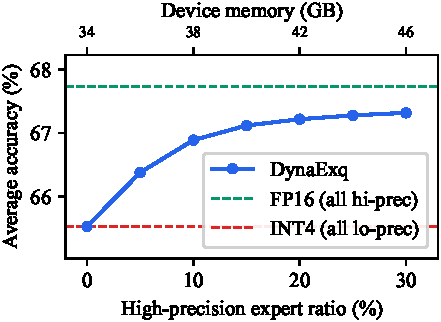
\includegraphics[width=0.48\columnwidth]{figures/budget_sensitivity_qwen30b.pdf}%
  }
  \hfill
  \subfloat[Qwen3-Next-80B]{%
    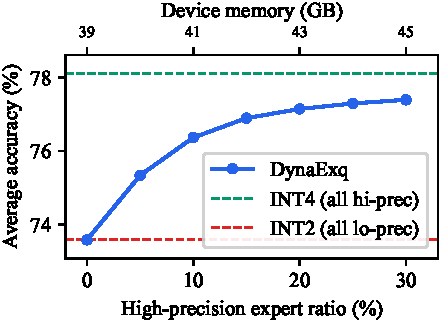
\includegraphics[width=0.48\columnwidth]{figures/budget_sensitivity_qwen80b.pdf}%
  }
  \caption{Average accuracy vs.\ high-precision expert budget ($n_{\mathrm{hi}}/E$). The dashed line marks the static all-low baseline at 0\%.}
  \label{fig:budget_sensitivity}
  \vspace{-1em}
\end{figure}

Both curves exhibit diminishing returns, consistent with a heavy-tailed routing distribution in which a small expert subset receives much of the traffic.

On Qwen3-30B the first 5\% of high-precision experts recovers 0.85\,pp of the 2.20\,pp FP16--INT4 gap, while the next 5\% adds only 0.51\,pp. Each upgrade adds 6.68\,MiB per expert under the packed layout, so the memory price of the first 5\% is already non-trivial. On Qwen3-Next-80B the effect is more pronounced: the first 5\% recovers 1.76\,pp of the 4.54\,pp INT4--INT2 gap, because the wider precision gap amplifies per-expert quality impact while each upgrade adds only 0.703\,MiB. Beyond 25\%, gains on both models fall below 0.1\,pp per 5\% increment. We stop the sweep at 30\% because Qwen3-30B already reaches 46.2\,GB at that point, leaving less than 2\,GB of headroom before the 48\,GB HBM ceiling.

\systemname's default of approximately 20\% lies near the observed knee for both models, recovering 77--79\% of the respective accuracy gap while using 42--43\,GB of the 48\,GB envelope. This shared ratio is descriptive rather than evidence of precision-independent policy optimality. The sweep instead provides a deployment tradeoff: on Qwen3-30B, reducing the ratio from 20\% to 10\% costs approximately 0.33 percentage points while releasing about 4\,GB for other serving state, such as the KV cache.

\section{Related Work}

Prior work exposes three complementary control variables for memory-constrained MoE inference: expert placement, offline precision assignment, and hybrid movement/compression. \systemname\ explores a fourth operating point: every routed expert remains device-addressable, while the identities occupying fixed higher-precision slots change online. The contribution is therefore not mixed precision or utilization scoring alone, but a fully resident replacement protocol with versioned publication, admission-before-allocation, and bounded resident/staging pools.

\begin{table}[!h]
\centering
\caption{Mechanism boundary relative to representative baselines. A routed cache miss may require host-to-device transfer even when prefetch hides some or all of its latency.}
\label{tab:mechanism_boundary}
\vspace{-0.4em}
\scriptsize
\setlength{\tabcolsep}{2.2pt}
\resizebox{\columnwidth}{!}{%
\begin{tabular}{lccc}
\toprule
\textbf{System} & \textbf{Device expert state} & \textbf{Online control target} & \textbf{Routed miss transfer} \\
\midrule
Uniform PTQ & Complete, fixed & None (offline map) & No \\
MoE-Infinity~\cite{xue2024moe} & Partial GPU cache & Placement/prefetch & Possible \\
HOBBIT~\cite{tang2024hobbit} & Partial GPU cache & Miss precision + placement & Possible \\
ExpertFlow~\cite{shen2025expertflow} & Partial GPU cache & Prefetch/routing & Possible \\
\systemname & Complete, versioned & Precision residency & No \\
\bottomrule
\end{tabular}}
\end{table}

\subsection{MoE Offloading and Memory Hierarchy Management}
General-purpose LLM inference engines such as vLLM~\cite{kwon2023vllm}, SGLang~\cite{zheng2024sglang}, and FlexGen~\cite{sheng2023flexgen} manage KV-cache memory, request scheduling, or model offloading. MoE-specific systems additionally exploit routed access: Adaptive gating~\cite{li2023adaptive}, EdgeMoE~\cite{yi2023edgemoe}, MoE-Infinity~\cite{xue2024moe}, Mixtral-offloading~\cite{eliseev2023fast}, Pre-gated MoE~\cite{hwang2024pre}, AdaMoE~\cite{zhong2024adapmoe}, ProMoE~\cite{song2024promoe}, and ExpertFlow~\cite{shen2025expertflow} differ in prediction, staging, and coordination but primarily control \emph{placement} and \emph{fetch time} (\autoref{tab:mechanism_boundary}). MoE-Infinity builds a locality-aware offload cache, ProMoE proactively schedules fixed-precision weights, and ExpertFlow adapts its prediction horizon and cache coordination. \systemname\ removes routed cache misses by keeping a complete expert set in HBM and instead controls the precision of resident experts.

\subsection{Static PTQ and Generic Low-Bit Inference}
Weight-only and activation-aware PTQ schemes such as GPTQ~\cite{frantar2022gptq}, AWQ~\cite{lin2024awq}, and LLM.int8()~\cite{dettmers2022gptint8} improve accuracy at aggressive bitwidths but produce a \emph{static} precision configuration. Even methods that adapt bit choices at calibration time deploy a fixed precision map at inference. Theoretically grounded expert-wise allocation~\cite{chowdhury2026efficient} further improves static assignments using router change and quantization-noise proxies. These methods are complementary sources of offline sensitivity priors; they do not define a concurrent online replacement protocol.

\subsection{MoE-Specific Mixed Precision}
MxMoE~\cite{duanmu2025mxmoe} derives mixed-precision configurations from expert sensitivity and couples them with mixed-precision grouped GEMMs. MoPEQ~\cite{chitty2025mopeq} assigns bitwidths using activation frequency and sensitivity measures. Earlier work on routing stability~\cite{fedus2022switch} and expert specialization~\cite{dai2024deepseekmoe} explored how expert heterogeneity affects model quality, providing motivation for non-uniform precision allocation. These methods improve the quality--memory tradeoff at model-build time. MxMoE, for example, produces mixed-precision kernels but assigns bitwidths statically with no runtime residency control. The resulting precision map stays \emph{fixed} during inference and does not adapt as routing distributions shift.

\subsection{Hybrid Systems}
HOBBIT~\cite{tang2024hobbit} combines mixed-precision representations with offloading to reduce cache-miss transfer cost, demonstrating that precision and placement can be optimized jointly. DyMoE~\cite{huang2026dymoe} dynamically classifies experts, applies depth-aware 8/4/0-bit policies, and prefetches missing versions from CPU or SSD for 12--24\,GB edge devices. \systemname\ targets a different capacity regime and invariant: on a 48\,GB GPU it keeps one version of every routed expert resident, uses long-horizon router statistics, and replaces representations through leases, last-use events, publish-after-copy handles, and byte-level admission control. DyMoE's phase-aware placement policy and \systemname's resident replacement mechanism are potentially complementary; comparing them on common models and hardware remains future work.

\section{Limitations and Scope}
\label{sec:limitations}

\systemname\ has five principal limitations. First, it keeps kernel-ready high- and low-precision expert representations in host memory. This removes online repacking from the critical path but increases pinned-DRAM demand and may be unsuitable for edge hosts with limited memory. Disk-backed preparation would reduce DRAM use at the cost of another latency tier.

Second, the current policy optimizes aggregate routing utility. It does not provide per-tenant quality guarantees or fairness when concurrent requests have different domains. Per-request precision decisions would also make batching less regular. Extending the objective with tenant weights or service-level constraints is therefore a policy problem that the present mechanism does not solve.

Third, our evaluation covers one 48\,GB GPU and three model families. Transfer/compute overlap and the feasible high-precision capacity depend on the GPU, PCIe generation, sequence length, and KV-cache policy, so the operating points are platform measurements. The pinned MoE-Infinity open-source runtime supports Qwen3-30B but not the other two checkpoints, and it differs from the implementation in its paper. The design uses two precomputed tiers on one GPU and a fixed task order.

Fourth, the prototype favors correctness and inspectability over kernel maturity. Handle-aware dispatch currently uses eager expert execution for Qwen-family models because the upstream grouped-GEMM shortcut does not accept per-expert versioned handles. This isolates the systems effect under study but leaves integration with a fused handle-aware grouped kernel to future work. Dual-tier packing and pinned-host-cache construction are untimed startup costs; production deployments would need to amortize or persist this preparation.

Finally, the hard invariant applies to \systemname-owned expert pools, staging blocks, and declared conversion workspace. End-to-end device-memory safety is conditional on the serving configuration keeping KV-cache, activation, and framework allocations within their startup reservations; the prototype does not replace or police the framework allocator. A separate CUDA stream removes explicit migration synchronization from the forward path but cannot eliminate resource contention: copies and repacking kernels may still share memory-system bandwidth with inference. Our latency scope is an isolated model and excludes request queueing, tokenization, network transport, and serialization. We therefore compare model-level end-to-end and tail latency, not only scheduler CPU time.

\section{Conclusion}

\systemname\ manages expert precision online within an explicit memory envelope. Routing statistics allocate high-precision capacity, while versioned handles, admission control, and fixed-block pools replace representations atomically. Separating policy from mechanism recovers much of the quality lost to uniform low-bit quantization without expert offloading's batch-dependent transfers. Future work should reduce host duplication and coordinate quality and memory budgets across tenants and GPUs.


\bibliographystyle{IEEEtran}
\bibliography{references}

\end{document}
